\documentclass{article}
\usepackage{tikz}
\usepackage{xcolor}
\usetikzlibrary{shapes,arrows,positioning,fit,backgrounds}

\begin{document}

\begin{figure}[htbp]
\centering
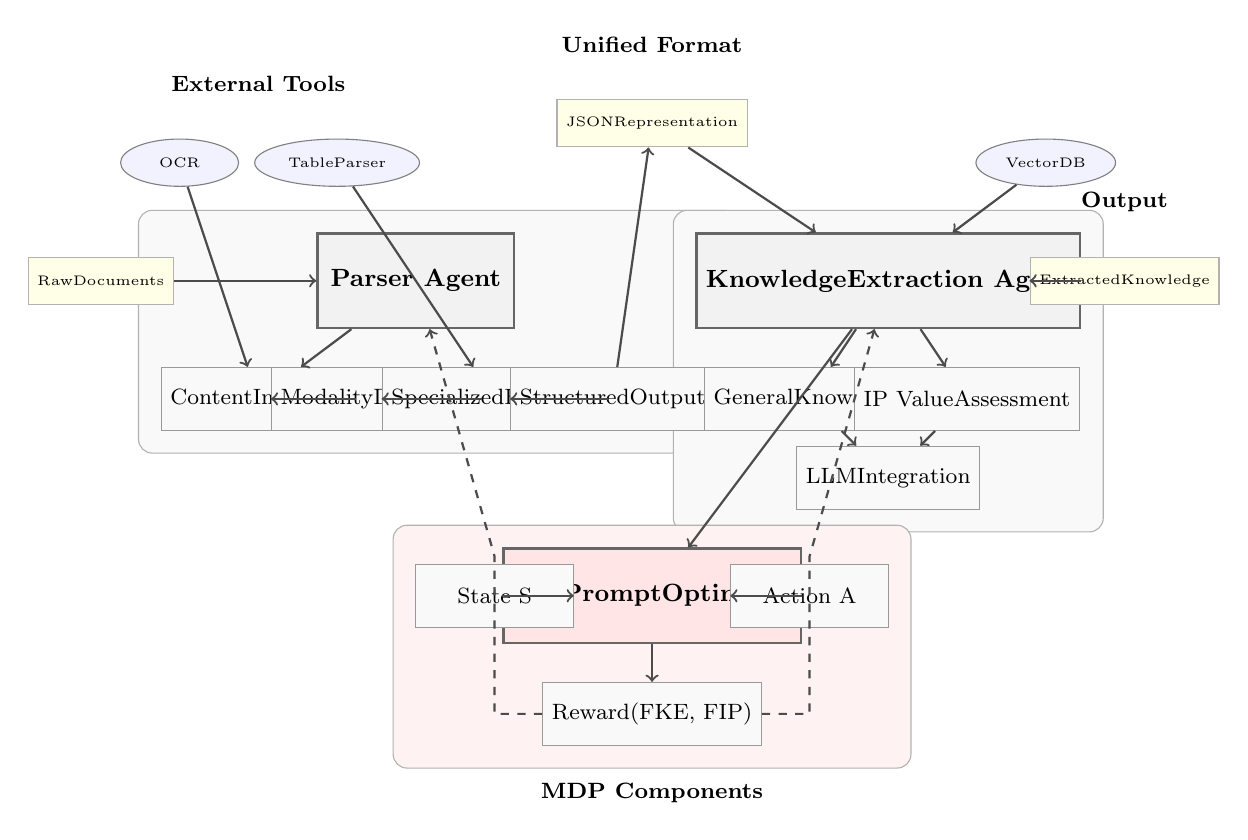
\begin{tikzpicture}[
    % Define styles
    agent/.style={rectangle, draw=black!60, fill=gray!10, thick, minimum width=2.5cm, minimum height=1.2cm, text centered, font=\small\bfseries},
    submodule/.style={rectangle, draw=black!40, fill=gray!5, minimum width=2cm, minimum height=0.8cm, text centered, font=\footnotesize},
    tool/.style={ellipse, draw=black!50, fill=blue!5, minimum width=1.5cm, minimum height=0.6cm, text centered, font=\tiny},
    arrow/.style={->, thick, black!70},
    data/.style={rectangle, draw=black!30, fill=yellow!10, minimum width=1.8cm, minimum height=0.6cm, text centered, font=\tiny},
    rl/.style={rectangle, draw=black!60, fill=red!10, thick, minimum width=2.5cm, minimum height=1.2cm, text centered, font=\small\bfseries}
]

% Main Agents
\node[agent] (parser) at (0,4) {Parser Agent};
\node[agent] (knowledge) at (6,4) {Knowledge\\Extraction Agent};
\node[rl] (rl) at (3,0) {RL Prompt\\Optimizer};

% Parser Agent Sub-processes
\node[submodule] (ingestion) at (-2,2.5) {Content\\Ingestion};
\node[submodule] (detection) at (-0.5,2.5) {Modality\\Detection};
\node[submodule] (handling) at (1,2.5) {Specialized\\Handling};
\node[submodule] (output) at (2.5,2.5) {Structured\\Output};

% Knowledge Extraction Sub-processes
\node[submodule] (general) at (5,2.5) {General\\Knowledge};
\node[submodule] (ip) at (7,2.5) {IP Value\\Assessment};
\node[submodule] (llm) at (6,1.5) {LLM\\Integration};

% External Tools
\node[tool] (ocr) at (-3,5.5) {OCR};
\node[tool] (table) at (-1,5.5) {Table\\Parser};
\node[tool] (vector) at (8,5.5) {Vector\\DB};

% Data Flow
\node[data] (raw) at (-4,4) {Raw\\Documents};
\node[data] (json) at (3,6) {JSON\\Representation};
\node[data] (extracted) at (9,4) {Extracted\\Knowledge};

% RL Components
\node[submodule] (state) at (1,0) {State S};
\node[submodule] (action) at (5,0) {Action A};
\node[submodule] (reward) at (3,-1.5) {Reward\\(FKE, FIP)};

% Connections
% Raw documents to Parser Agent
\draw[arrow] (raw) -- (parser);

% Parser Agent internal flow
\draw[arrow] (parser) -- (ingestion);
\draw[arrow] (ingestion) -- (detection);
\draw[arrow] (detection) -- (handling);
\draw[arrow] (handling) -- (output);

% External tools to Parser
\draw[arrow] (ocr) -- (ingestion);
\draw[arrow] (table) -- (handling);

% Parser to Knowledge Extraction
\draw[arrow] (output) -- (json);
\draw[arrow] (json) -- (knowledge);

% Knowledge Extraction internal
\draw[arrow] (knowledge) -- (general);
\draw[arrow] (knowledge) -- (ip);
\draw[arrow] (general) -- (llm);
\draw[arrow] (ip) -- (llm);

% External tools to Knowledge Extraction
\draw[arrow] (vector) -- (knowledge);

% Knowledge Extraction output
\draw[arrow] (knowledge) -- (extracted);

% RL connections
\draw[arrow] (knowledge) -- (rl);
\draw[arrow] (rl) -- (state);
\draw[arrow] (rl) -- (action);
\draw[arrow] (rl) -- (reward);

% Feedback loop
\draw[arrow, dashed] (reward) -- ++(-2,0) -- ++(0,2) -- (parser);
\draw[arrow, dashed] (reward) -- ++(2,0) -- ++(0,2) -- (knowledge);

% Background boxes for grouping
\begin{scope}[on background layer]
    \node[fit=(parser)(ingestion)(detection)(handling)(output), draw=black!30, fill=gray!5, rounded corners=5pt, inner sep=8pt] {};
    \node[fit=(knowledge)(general)(ip)(llm), draw=black!30, fill=gray!5, rounded corners=5pt, inner sep=8pt] {};
    \node[fit=(rl)(state)(action)(reward), draw=black!30, fill=red!5, rounded corners=5pt, inner sep=8pt] {};
\end{scope}

% Labels
\node[font=\footnotesize] at (-2,6.5) {\textbf{External Tools}};
\node[font=\footnotesize] at (3,7) {\textbf{Unified Format}};
\node[font=\footnotesize] at (9,5) {\textbf{Output}};
\node[font=\footnotesize] at (3,-2.5) {\textbf{MDP Components}};

\end{tikzpicture}
\caption{System Architecture Overview: Three-module framework with Parser Agent, Knowledge Extraction Agent, and RL Prompt Optimizer forming a closed-loop workflow.}
\label{fig:architecture}
\end{figure}

\end{document}